% =========================================================================
% MÓDULO 1: PORTADA, AGENDA TT2, OBJETIVOS Y CONTEXTO DE VALIDACIÓN (DIAPS. 1 A 5)
% =========================================================================

% --- DIAPOSITIVA 1: PORTADA INSTITUCIONAL ---
\begin{frame}[t]
  \vspace{1mm}
  \begin{columns}[c,onlytextwidth]
    \begin{column}{0.14\textwidth}
      \centering
      
\includegraphics[height=1.65cm,keepaspectratio]{imgs/ipn.jpg}
    \end{column}
    \begin{column}{0.70\textwidth}
      \centering
      {\footnotesize\bfseries\textcolor{ipnDark}{INSTITUTO POLIT\'ECNICO NACIONAL}}\\[1mm]
      {\scriptsize\bfseries\textcolor{textDark}{ESCUELA SUPERIOR DE C\'OMPUTO (ESCOM)}}\\[0.8mm]
      {\scriptsize\textcolor{textMuted}{Ingenier\'ia en Inteligencia Artificial}}
    \end{column}
    \begin{column}{0.14\textwidth}
      \centering
      
\includegraphics[height=1.55cm,keepaspectratio]{imgs/escom.png}
    \end{column}
  \end{columns}

  \vspace{2mm}
  \begin{beamercolorbox}[rounded=true,sep=3mm]{palette primary}
    \centering
    {\normalsize\bfseries Optimizaci\'on bayesiana de redes neuronales para la decodificaci\'on de movimientos de los dedos a partir de se\~nales electrocorticogr\'aficas}\\[2mm]
    {\scriptsize\textcolor{ipnAccent}{\textbf{Defensa de Trabajo Terminal II}} \quad|\quad Registro Oficial: \textbf{2026-B145}}
  \end{beamercolorbox}

  \vspace{2.5mm}
  \begin{columns}[T,onlytextwidth]
    \begin{column}{0.48\textwidth}
      \begin{block}{Autores que Presentan}
        \footnotesize
        \begin{itemize}\setlength{\itemsep}{2pt}
          \item \textbf{Saul Rodas Bautista}
          \item \textbf{Joel Valencia San Roman}
        \end{itemize}
      \end{block}
    \end{column}
    \begin{column}{0.48\textwidth}
      \begin{block}{Directores del Trabajo Terminal}
        \footnotesize
        \begin{itemize}\setlength{\itemsep}{2pt}
          \item \textbf{Dra.\ Miriam Pescador Rojas}
          \item \textbf{M.C.\ Miguel Abel Le\'on Hern\'andez}
        \end{itemize}
      \end{block}
    \end{column}
  \end{columns}
\end{frame}

% --- DIAPOSITIVA 2: PROBLEMÁTICA DEL PROYECTO ---
\begin{frame}{Problem\'atica del Proyecto}{Variabilidad inter-sujeto, costo computacional y decodificaci\'on cinem\'atica continua \cite{miller2008prediction}}
  \begin{columns}[T,onlytextwidth]
    \begin{column}{0.48\textwidth}
      \begin{block}{Calidad de Se\~nales y Tarea Motora}
        \scriptsize
        El desarrollo de interfaces cerebro-computadora de alta precisi\'on depende de la calidad de las se\~nales capturadas y de la capacidad de interpretar los patrones neuronales asociados al movimiento. En este estudio, se utilizan se\~nales de electrocorticograf\'ia (ECoG) del Data Set 4 de la BCI Competition IV, las cuales permiten estudiar la relaci\'on entre la actividad cerebral y las trayectorias continuas de flexi\'on de los dedos \cite{miller2008prediction}.
      \end{block}
      \vspace{1.5mm}
      \begin{block}{Variabilidad Inter-Sujeto y Redes Profundas}
        \scriptsize
        Uno de los principales desaf\'ios en el procesamiento de estas se\~nales es la diferencia en la cantidad de canales y en la ubicaci\'on de los electrodos entre sujetos. Esta variabilidad dificulta la construcci\'on de un modelo de aprendizaje preciso para todos los casos. Para interpretar estas se\~nales complejas, las redes neuronales profundas representan una herramienta \'util; no obstante, su eficacia depende en gran medida de la configuraci\'on de su arquitectura y de sus hiperpar\'ametros.
      \end{block}
    \end{column}

    \begin{column}{0.48\textwidth}
      \begin{block}{Costo Computacional y Optimizaci\'on Bayesiana}
        \scriptsize
        Al explorar diferentes combinaciones posibles, se requiere una capacidad computacional considerable, ya que cada configuraci\'on puede necesitar un nuevo entrenamiento. Incluso con otros m\'etodos de b\'usqueda, como los algoritmos bioinspirados, este proceso puede resultar complejo y costoso. Por ello, surge la necesidad de estudiar la optimizaci\'on bayesiana como una alternativa para realizar una b\'usqueda inteligente, basada en modelos probabil\'isticos, dentro del espacio de configuraciones de la red neuronal.
      \end{block}
      \vspace{1.5mm}
      \begin{alertblock}{Problema Central y Propuesta de Soluci\'on}
        \scriptsize
        El problema central reside en determinar qu\'e configuraciones de arquitectura e hiperpar\'ametros permiten obtener una mayor precisi\'on en la predicci\'on de las trayectorias continuas de flexi\'on de los dedos, considerando las diferencias entre los datos de cada sujeto. Para ello, se propone desarrollar un marco de configuraci\'on basado en redes neuronales profundas y optimizaci\'on bayesiana, cuyo desempe\~no ser\'a evaluado mediante la correlaci\'on entre los movimientos predichos y los reales, y comparado con el modelo base y con los resultados reportados en la literatura.
      \end{alertblock}
    \end{column}
  \end{columns}
\end{frame}

% --- DIAPOSITIVA 3: OBJETIVO GENERAL, OBJETIVOS PARTICULARES Y PROPUESTA DE SOLUCIÓN ---
\begin{frame}{Objetivo General, Objetivos Particulares y Propuesta de Soluci\'on}
  \begin{alertblock}{Objetivo General}
    \footnotesize
    Desarrollar un marco de configuraci\'on basado en redes neuronales profundas para la decodificaci\'on continua de movimientos de dedos a partir de se\~nales electrocorticogr\'aficas del Dataset 4 de la BCI Competition IV, optimizando su arquitectura e hiperpar\'ametros mediante optimizaci\'on bayesiana y comparando su desempe\~no frente al modelo base y al estado del arte.
  \end{alertblock}

  \vspace{2mm}
  \begin{columns}[T,onlytextwidth]
    \begin{column}{0.48\textwidth}
      \begin{block}{Objetivo Particular 1}
        \scriptsize
        Implementar una metodolog\'ia de filtrado, segmentaci\'on, normalizaci\'on y extracci\'on espectral libre de fuga de informaci\'on temporal.
      \end{block}
      \vspace{2mm}
      \begin{block}{Objetivo Particular 2}
        \scriptsize
        Integrar el flujo continuo de modelado dise\~nando una arquitectura base y su evoluci\'on estructural para predecir trayectorias de flexi\'on.
      \end{block}
    \end{column}

    \begin{column}{0.48\textwidth}
      \begin{block}{Objetivo Particular 3}
        \scriptsize
        Dise\~nar e implementar con Optuna un esquema de optimizaci\'on bayesiana para buscar autom\'aticamente arquitecturas e hiperpar\'ametros por sujeto.
      \end{block}
      \vspace{2mm}
      \begin{block}{Objetivo Particular 4}
        \scriptsize
        Comparar el modelo optimizado frente al modelo base y al estado del arte bajo condiciones auditables.
      \end{block}
    \end{column}
  \end{columns}
\end{frame}

% --- DIAPOSITIVA 4: RECUERDO DEL TRABAJO TERMINAL 1: CONTEXTO DE LA MUESTRA ---
\begin{frame}{Recuerdo del Trabajo Terminal 1: contexto de la muestra}{Heterogeneidad anat\'omica de los tres sujetos en el \textit{Dataset 4} (\textit{BCI Competition IV}) \cite{miller2008prediction,schalk2004bci2000,Schalk2011}}
  \vfill
  \centering
  {\small
  \renewcommand{\arraystretch}{1.28}
  \setlength{\tabcolsep}{6pt}
  \begin{tabularx}{\textwidth}{@{} l c c c >{\raggedright\arraybackslash}X @{}}
    \toprule
    \rowcolor{ipnDark}
    \textcolor{white}{\textbf{Sujeto}} &
    \textcolor{white}{\textbf{Canales V\'alidos}} &
    \textcolor{white}{\textbf{Desarrollo (CV)}} &
    \textcolor{white}{\textbf{Prueba Oficial}} &
    \textcolor{white}{\textbf{Condici\'on Anat\'omica y Relaci\'on Se\~nal-Ruido}} \\
    \midrule
    \textbf{Sujeto 1 (\texttt{S1})} & $61\text{ electrodos}$ & $400\text{ s}$ ($5\text{ bloques}$) & $200\text{ s}$ & Cobertura fronto-parietal est\'andar con acoplamiento moderado entre dedos. \\
    \rowcolor{rowHighlight}
    \textbf{Sujeto 2 (\texttt{S2})} & $46\text{ electrodos}$ & $400\text{ s}$ ($5\text{ bloques}$) & $200\text{ s}$ & Menor densidad espacial de rejilla y menor relaci\'on se\~nal-ruido basal. \\
    \textbf{Sujeto 3 (\texttt{S3})} & $63\text{ electrodos}$ & $400\text{ s}$ ($5\text{ bloques}$) & $200\text{ s}$ & Cobertura densa sobre el giro precentral (M1) con alta selectividad motora. \\
    \bottomrule
  \end{tabularx}
  }
  \fuente{Creaci\'on propia a partir de \cite{miller2008prediction,Schalk2011} y el repositorio GitHub \cite{rodas_valencia_tpe_ecog}.}

  \vspace{1.5mm}
  \begin{beamercolorbox}[rounded=true,sep=1.5mm]{block body alerted}
    \scriptsize\centering
    \textbf{Enfoque TT2:} Redise\~no Arquitect\'onico (\texttt{A1--A5}) \ \textbullet\ Optuna \textbf{TPE} \ \textbullet\ $723$ Entrenamientos Verificados
  \end{beamercolorbox}
  \vfill
\end{frame}

% --- DIAPOSITIVA 5: CONTEXTO METODOLÓGICO II: DIVISIÓN DE LOS BLOQUES DE VALIDACIÓN ---
\begin{frame}{Procedimiento de Validaci\'on: Divisi\'on en Cinco Bloques}{Partici\'on cronol\'ogica con zona de purga para impedir fuga de informaci\'on temporal \cite{roberts2017crossvalidation,rodas_valencia_tpe_ecog}}
  \begin{columns}[c,onlytextwidth]
    \begin{column}{0.40\textwidth}
      \begin{block}{Esquema de Validaci\'on Cruzada ($K = 5$)}
        \scriptsize
        \begin{itemize}\setlength{\itemsep}{3pt}
          \item \textbf{Cinco bloques cronol\'ogicos (\texttt{B1--B5}):} Los $400\text{ s}$ de desarrollo se dividen en $5$ bloques contiguos de $N = 7750$ muestras v\'alidas a $100\text{ Hz}$ cada uno.
          \item \textbf{Rotaci\'on de pliegues:} En cada pliegue $k \in \{1,\dots,5\}$, un bloque completo act\'ua como validaci\'on y los $4$ restantes como entrenamiento.
          \item \textbf{Margen de purga ($\mathbf{P = 256}$):} Con ventanas deslizantes de $W=256$ muestras ($2.56\text{ s}$), se aplica una separaci\'on de $256$ muestras para garantizar \textbf{solapamiento cero ($\mathbf{0.0}$)} entre entrenamiento y validaci\'on \cite{roberts2017crossvalidation}.
        \end{itemize}
      \end{block}
    \end{column}

    \begin{column}{0.57\textwidth}
      \centering
      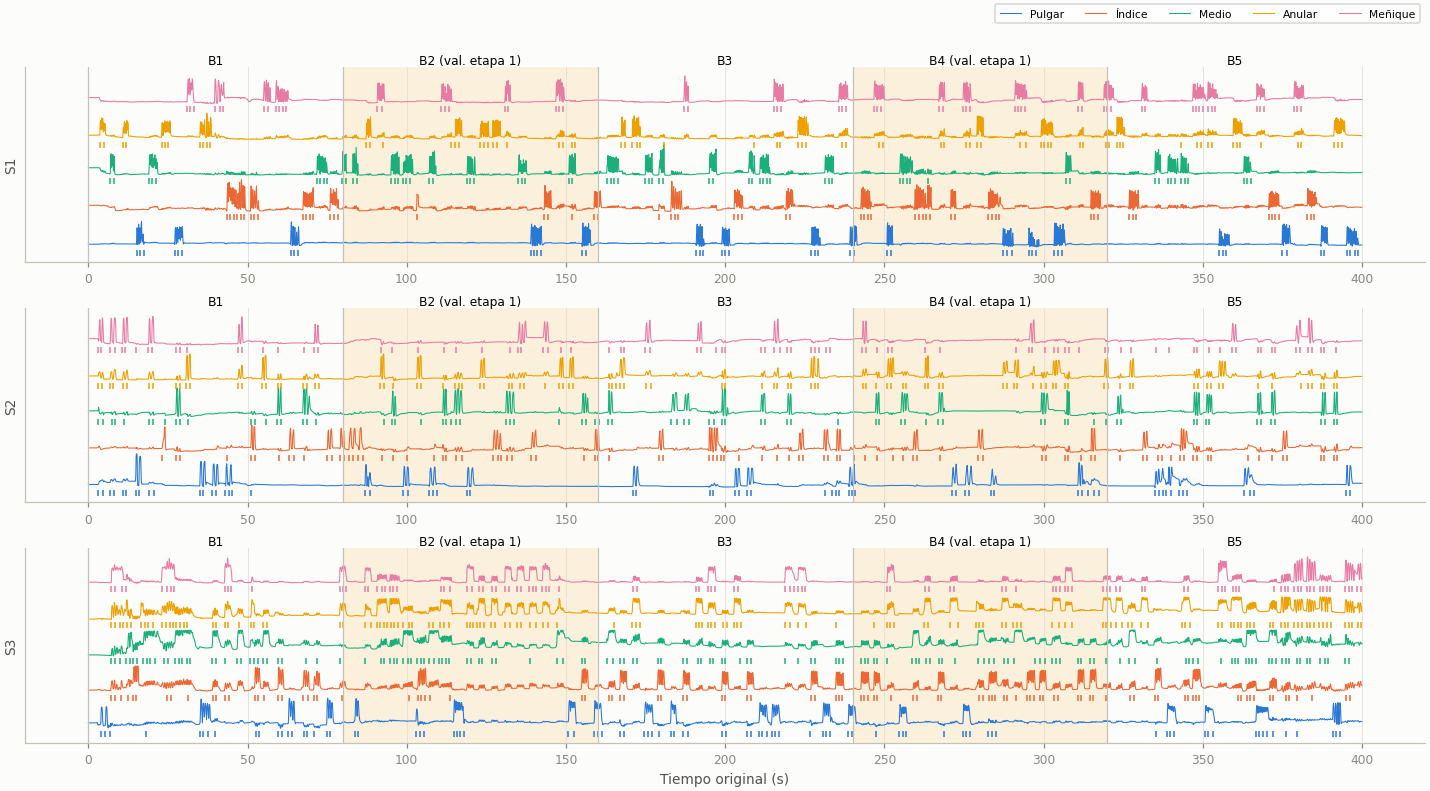
\includegraphics[width=\linewidth,height=0.47\textheight,keepaspectratio]{imgs/s11_blocks_timeline.png}
      \figcap{1}{Divisi\'on de la se\~nal en cinco bloques cronol\'ogicos (\texttt{B1--B5}) y zona de purga ($P=256$ muestras) empleada en todos los experimentos de TT2. \textbf{Fuente:} Obtenida del repositorio GitHub \cite{rodas_valencia_tpe_ecog}.}
    \end{column}
  \end{columns}

  \takeaway{Esta divisi\'on por bloques purgados garantiza que tanto las ablaciones arquitect\'onicas como la b\'usqueda en Optuna TPE eval\'uen la generalizaci\'on real sobre intervalos futuros no observados \cite{roberts2017crossvalidation,rodas_valencia_tpe_ecog}.}
\end{frame}
